\documentclass[12pt]{article}
\usepackage{amsmath}
\usepackage{times}
\usepackage[top=1.0in, bottom=0.9in, left=0.9in, right=0.7in]{geometry}


\usepackage{float}
\usepackage{graphicx}
\usepackage{subfig}
\usepackage{wrapfig,lipsum}
\usepackage{amssymb}
\usepackage{amsfonts}
\usepackage{mleftright}
\usepackage{hhline}

% For matlab code typesetting https://www.mathworks.com/matlabcentral/fileexchange/8015-m-code-latex-package
\usepackage[framed,numbered,autolinebreaks,useliterate]{mcode}








\begin{document}

\title{Math 226A - HW1}
\author{Ahmed H. Mahmoud}
\date{October, 13th 2017} 

\maketitle

\newcommand{\cn}{Crank-Nicolson}

\section*{Problem No.1} \label{sec:prob1}

An iteration of Newton's method is 
\[
x_{k+1} = x_{k} - \frac{f(x_{k})}{f^{\prime}(x_{k})} 
\]

We can subtract $x_{*}$ from both sides and rearrange. We then get
\begin{equation}
\frac{x_{k+1} -x_{*}}{x_{k} -x_{*}} = 1 - \frac{f(x_{k})}{f^{\prime}(x_{k}) (x_{k}-x_{*})} 
\end{equation}


We can use Taylor expansion to express $f(x_{k})$ and $f^{\prime}(x_{k})$ in terms of $f(x_{*})$ and higher order terms as follows
\[
f(x) = f(x_{*}) + f^{\prime}(x_{*})(x-x_{*}) + \frac{f^{\prime \prime}(x_{*})}{2}(x-x_{*})^{2}+HOT 
\] 
where $HOT$ stands for \emph{higher order terms}. Since $f(x)=f^{\prime}(x)=0$, we get
\begin{equation}
f(x) = \frac{f^{\prime \prime}(x_{*})}{2}(x-x_{*})^{2}+HOT
\end{equation}
We can differentiate (2) once about $x$. We get
\begin{equation}
f^{\prime}(x) = f^{\prime \prime}(x_{*})(x-x_{*})+HOT
\end{equation}

We can then evaluate (2) and (3) at $x_{k}$ and substitute in (1) to get
\[
\frac{x_{k+1} -x_{*}}{x_{k} -x_{*}} = 1 - \frac{  \frac{f^{\prime \prime}(x_{*})}{2}(x_{k}-x_{*})^{2}+HOT }{ (f^{\prime \prime}(x_{*})(x_{k}-x_{*})+HOT) (x_{k}-x_{*})}
\]
\[
\frac{x_{k+1} -x_{*}}{x_{k} -x_{*}} = 1 - \frac{1}{2} \left( \frac{1}{1 + HOT*(f^{\prime \prime}(x_{*})(x_{k}-x_{*}))^{-1}}\right)
\]
Taking the limits as $k\rightarrow \infty$ in the last expression, the higher order terms will go to zero and we get 
$$
\lim_{k \to \infty} \frac{x_{k+1} -x_{*}}{x_{k} -x_{*}} = \lim_{k \to \infty} \frac{e_{k+1}}{e_{k}} = \frac{1}{2} \qquad \qquad \qquad \blacksquare
$$

\newpage

\section*{Problem No.2} \label{sec:prob2}
\paragraph{Part (a):} 
Due to the inexact representation of number using the IEEE standards in MATLAB, summing or subtracting numbers that are too close to one another will produce erroneous results depending on the relative error. The relative error or $\epsilon_{machine}$ is defined as 
$$
\frac{|fl(x)-x|}{|x|} \leq \frac{2^{m-k}}{|x|}
$$
where $fl(x)$ is the floating-point representation of $x$ $m$ is the number of bits used for the exponent and $k$ is number of bits used for the mantissa. For double precision, MATLAB $\epsilon_{machine}=2.2\times10^{-16}$ means if two numbers have the same 16 digits after the floating point, then the computer will store them as the same number. Using WolframAlpha which uses much lower $\epsilon_{machine}$ and can represent numbers more accurately, we get
$$
atan(x+1) = 1.570796316794896719231321024973084775431998033019552910498\\
$$
$$
atan(x)=1.570796316794896619231322024973084775431898033020886243822
$$
for $x=10^8$ which differ after the 47th digit. This explains why MATLAB calculates $I(x)$ to be 0 for $x=10^8$.
 
\paragraph{Part (b):} 

$I(x)$ can be evaluated as follows:
\[
I(x) = \int_{x}^{x+1} \frac{1}{1+s^2} ds = \int_{x}^{x+1} \frac{1}{s-i} \frac{1}{s+i}ds
\]
$$
I(x) = \frac{1}{2i}  \left( \int_{x}^{x+1} \frac{1}{s-1} ds- \int_{x}^{x+1} \frac{1}{s+i} ds \right)
$$
$$
I(x) = \frac{1}{2i}  \left( ln(s-i) - ln(s+i) \right)_{x}^{x+1}
$$
$$
I(x) = \frac{1}{2i}  \left( ln\left(\frac{x+1-i}{x+1+i}\right) - ln\left(\frac{x-i}{x+i}\right)\right)
$$


\paragraph{Part (c):} The above formula is implemented using the following MATLAB code:

\begin{lstlisting}
values = zeros(2,10);
for i=1:12
    x = power(10,i-1);
    values(1,i) = atan(x+1) - atan(x);
    values(2,i) = (1/2i)*(log((x+1-1i)/(x+1+1i)) - log((x-1i)/(x+1i)));
end
\end{lstlisting}

Using the above formula gives more accurate evaluation for $I(x)$ for large values of $x$. The following table shows a comparsion between the two formulae

%============table========
\begin{figure}[tbh]
 \centering  
  
\begin{tabular}{ |p{2cm}|| p{7cm}|p{7cm}|}
 \hline
 $x$ &  $I(x)=arctan(x+1) - arctan(x)$  & $I(x) = \frac{1}{2i}  \left( ln\left(\frac{x+1-i}{x+1+i}\right) - ln\left(\frac{x-i}{x+i}\right)\right)$ \\ \hhline{|=|=|=|}
 $10^0$          &$0.3217$        &$0.3217$ \\
 \hline
 $10^1$          &$0.009$        &$0.009 + 5.551\times 10^{-17}i$ \\
 \hline
 $10^2$          &$9.9 \times 10^{-05}$        &$9.9\times 10^{-05} - 5.55\times 10^{-17}i$ \\
 \hline
 $10^3$          &$9.99\times 10^{-07}$        &$9.99\times 10^{-07}$ \\
 \hline
 $10^4$          &$9.99\times 10^{-09}$        &$9.999\times 10^{-09}$ \\
 \hline
 $10^5$          &$9.999\times 10^{-11}$        &$9.999\times 10^{-11}$ \\
 \hline
 $10^6$          &$1.0\times 10^{-12}$        &$9.999\times 10^{-13}$ \\
 \hline
 $10^7$          &$9.99\times 10^{-15}$        &$9.999\times 10^{-15}$ \\
 \hline
 $10^8$          &$0$        &$9.999\times 10^{-17}$ \\
 \hline
 $10^9$          &$0$        &$1.0\times 10^{-18}$ \\
 \hline
 $10^10$         &$0$        &$1.0\times 10^{-20}$ \\
 \hline
 $10^10$         &$0$        &$9.999\times 10^{-23}$ \\
 \hline
 \hline

\end{tabular}
  \caption{Comparing the results of the two formulae of $I(x)$}
   
\end{figure} 
%============table========
While the logarithm formula works well, it was hard to find a good explanation on why it works. The only thing we can think of is that the computation of logarithm would split out the lose in precision into two numbers; real and imaginary part. Using WolframAlpha, we get 
$$		                                                                
 ln\left(\frac{x+1-i}{x+1+i}\right) = 18.42068076395236532214393 + 9.99999970000000566 \times 10^{-9}
$$
$$
 ln\left(\frac{x-i}{x+i}\right) = 18.42068074395236552214393+ 9.99999989999999966 \times 10^{-9}
$$
Both the real and imaginary parts starts to change after the 8th digits which is within MATLAB $\epsilon_{machine}$.



\newpage

\section*{Problem No.3} \label{sec:prob3}
Given the PDE along with boundary conditions 
\[
\epsilon u_{xx}-exp(-|u|)u+g =0,\\
u(0)=u(1)=0
\]
We can approximate the second derivative using the 3-point second-order discritzation 
\[
u_{xx}(x_{j}) \approx \frac{u_{j-1}-2u_{j}+u_{j+1}}{\Delta x^{2}}
\]
where $x_{j}=j\Delta x$ for $j=0 \cdots N+1$ and $\Delta x = \frac{1}{N+1}$ and thus $u_{j}\approx u(x_{j})$. The PDE then becomes 
\[
\frac{\epsilon}{\Delta x^{2}} \left(u_{j-1}-2u_{j}+u_{j+1}\right) - exp(-|u_{j}|)u_{j}+g=0
\]
When the problem is descrtized on $N$ mesh points, we will get $N-2$ in $N$  unknowns and the two boundary conditions will provide the additional two equations. The system of equations is nonlinear and Newton's method can be used to solved it by re-formulating the problem as solve for the roots of the following equation
\[
A(\overrightarrow{u}) + F(\overrightarrow{u})=0
\]
where $F(\overrightarrow{u}) = -exp(-|u_{j})u_{j}+g$ and 
\[
A = \frac{\epsilon}{\Delta x^{2}}
\left( 
\begin{array}{cc cc cc}
-2 & 1 &    &   &   & \\
1 & -2 & 1  &   &   & \\
  & \ddots & \ddots   & \ddots    &   & \\
  & & \ddots & \ddots   & \ddots   & \\
  &   &   & 1  & -2 &1 \\
  &   &   &    & 1 &-2 \\
\end{array} 
\right)
\]

In order to use Newton method, we estimated the Jacobian using finite difference. We note that the Jacobian is tridiagonal matrix and the code from \cite{doi:10.1137/1.9780898718898} is used in order to estimate the banded Jacobian efficiently where a column only needs three new function evaluations. 
\paragraph{Initial Guesses:} The first initial guess taken by considering $u$ and $u_{xx}$ are small and taking the limit $\epsilon =0$. Thus, the initial guess in that case is $u_{j}=g$ for $ j=2 \cdots N-1$ where $N$ is the total number of mesh points. The second initial guess is taken by considering $u$ is large and thus $exp(-|u|)$ is small. From that, we get the initial guess as $u_{j}=-\frac{1}{2}\frac{g}{\epsilon}x^{2}$.

Solving for these two initial guesses gave the solution as shown in Figure \ref{fig:prob3} left and middle for the first and second initial guess respectively. 

The third initial guess was found by taking weighted sum of the first two such that 
$u_{i3} = \alpha u_{i1} + (1-\alpha u_{i2})$ where $u_{i3}$ is the third initial guess we are looking for using the first initial guess $u_{i1}$ and second one $u_{i2}$ by doing binary search to find the right value of $\alpha$. Each iteration in the binary search would measure 2-norm of the obtain solution and update either the upper or lower bound of $\alpha$ (which are set initially to 1 and 0). The third solution was found with $\alpha = 0.999999098479748$ and shown in Figure \ref{fig:prob3} (right). 
 

\begin{figure}[H]
 \centering  
   {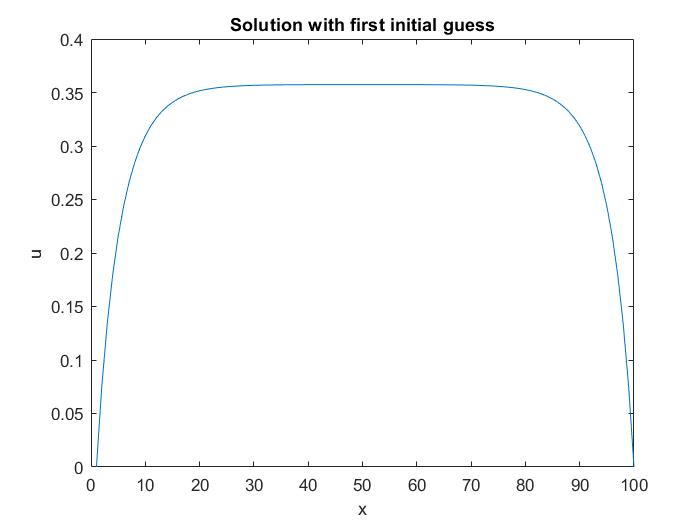
\includegraphics[width=0.32\linewidth]{code/p3_1.jpg}}   
   {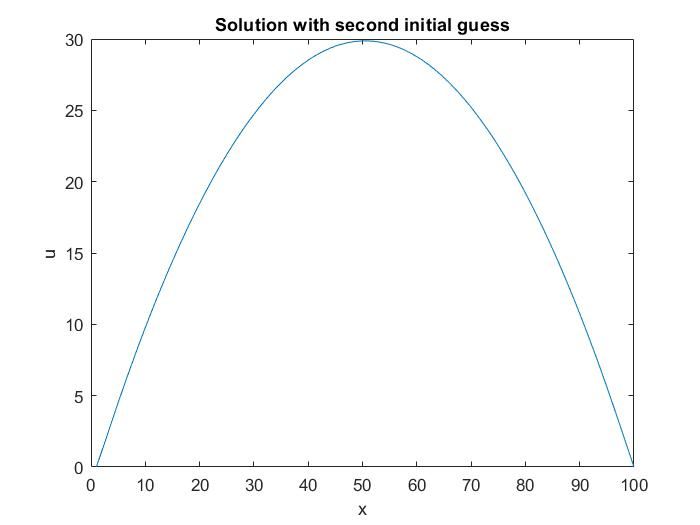
\includegraphics[width=0.32\linewidth]{code/p3_2.jpg}}
   {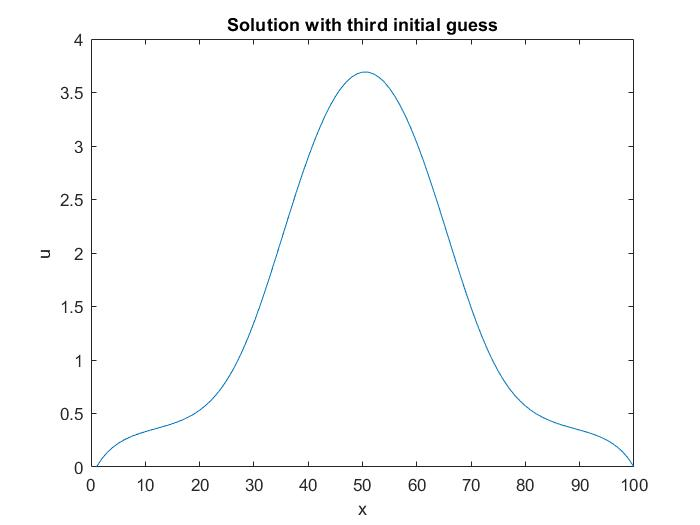
\includegraphics[width=0.32\linewidth]{code/p3_3.jpg}}
  \caption{The stable solutions for the nonlinear PDE defined in Problem No.3 where different initial guesses give different solutions. The nonlinear system of equations was solved using Newton method with Line Search on 100 mesh points.}
   \label{fig:prob3}
\end{figure} 


\newpage

\section*{Problem No.4} 
\paragraph{Part a:} The computes each sub-interval (.i.e, $a-c$ and $c-b$) twice; one before the refinement and one after. It would have been more efficient to pass this evaluation in the recursive call rather than computing them twice. 

\paragraph{Part b:}



\newpage

\section*{Appendix} \label{sec:app}

In problem 2, since $atan(x) = \frac{i}{2} ln \left( \frac{i+x}{i-x} \right)$, we can express the equation from question 2 as:
$$
atan(x+1) - atan(x)  =  \frac{i}{2}  \left( ln\left(\frac{i+x+1}{i-(x+1)}\right) - ln\left(\frac{i+x}{i-x}\right)\right) 
$$
We want to prove the following
\begin{equation}
\frac{1}{2i}  \left( ln\left(\frac{x+1-i}{x+1+i}\right) - ln\left(\frac{x-i}{x+i}\right)\right)  = \frac{i}{2}  \left( ln\left(\frac{i+x+1}{i-(x+1)}\right) - ln\left(\frac{i+x}{i-x}\right)\right) 
\end{equation}


such that the equation derived from the integration is correct.

\paragraph{Proof:}
Let 
$$
I_{1}(x) = \frac{1}{2i}  \left( ln\left(\frac{x+1-i}{x+1+i}\right) - ln\left(\frac{x-i}{x+i}\right)\right)
$$
we get
$$
I_{1}(x) = \frac{1}{2i} ln \left(\frac{(x+1-i)(x+i)}{(x+1+i)(x-i)} \right)
$$
$$
I_{1}(x) = \frac{1}{2i} ln \left( \frac{x^2 +x+1+i}{x^2+x+1-i} \right)
$$
$$
I_{1}(x) = \frac{1}{2}  ln \left( \frac{x^2 +x+1-i}{x^2+x+1+i}\right)^i
$$

We can express the RHS of (1) as 
$$
I_{2}(x) = \frac{i}{2}  \left( ln\left(\frac{i+x+1}{i-(x+1)}\right) - ln\left(\frac{i+x}{i-x}\right)\right) 
$$
$$
I_{2}(x) = \frac{i}{2} ln\left(\frac{(i+x+1)(i-x)}{(i-x-1)(i+x)}\right)
$$
$$
I_{2}(x) = \frac{i}{2} ln\left(\frac{x^2+x+1-i}{x^2+x+1+i}\right)
$$
$$
I_{2}(x) = \frac{1}{2} ln\left(\frac{x^2+x+1-i}{x^2+x+1+i}\right)^i
$$


%\bibliography{../mybib}
%\bibliographystyle{plain}
\end{document}